\chapter{Actionable Approximations of the Truth}\label{s:pck}

\begin{objectives}

\item
  Summarize research on how well learners are doing in introductory
  computing classes today.

\item
  Explain at least three factors that influence how well or how
  quickly people learn how to program, and give examples of each.

\item
  Summarize shortcomings in the ways that novices typically test their
  software.

\item
  Explain when and how to use program visualization to teach
  introductory programming courses.

\item
  Explain why tracing and explaining programs can be a more effective
  way to teach programming than having learners write programs.

\end{objectives}

\glossref{g:pedagogical-content-knowledge}{Pedagogical content
  knowledge} (PCK) is what stands between an instructor's knowledge of
the problem domain and their general knowledge of teaching.  In
computing, it includes things like what examples to use when teaching
how parameters are passed to a function, or what misconceptions about
nesting HTML tags are most common.  This chapter summarizes some of
the research-based pedagogical content knowledge we have about
teaching and learning programming; \cite{Sent2018} is an up-to-date
and more detailed exploration.

Computing education research is still a young discipline: the American
Society for Engineering Education was founded in 1893, the National
Council of Teachers of Mathematics in 1920, the American Association
of Physics Teachers in 1950---and the Computer Science Teachers
Association in 2005.  The simple truth is that We don't know as much
about how people learn to program as we do about how they learn to
read, play a sport, or do basic arithmetic.  However, we do know a few
things, and conferences like \href{http://sigcse.org/}{SIGCSE},
\href{http://iticse.acm.org/}{ITiCSE} and
\href{https://icer.hosting.acm.org}{ICER} are delivering a steady
stream of rigorous, insightful studies with immediate practical
application.

As with all research, some caution is required to interpret their
results.  Most of what is presented comes from studying school
children and university undergraduates, both because those are the
populations that researchers have easiest access to \cite{Henr2010},
and because those are the ages at which people most often learn to
program.  Less is known about adults learning to program in free-range
settings or about people who don't intend to be computer scientists,
but what we do know is included.  (For those interested in methods,
\cite{Ihan2016} summarizes the ones used most often in this kind of
research.)

Theories may change as more and better data becomes available, so if
this was an academic treatise, it would preface most claims with
statements like, ``Research may seem to indicate that{\ldots}''
However, as
\href{https://computinged.wordpress.com/2018/06/15/are-you-talking-to-me-interaction-between-teachers-and-researchers-around-evidence-truth-and-decision-making/}{Mark
  Guzdial wrote}, actual teachers in actual classrooms have to make
decisions regardless of whether research has clear answers yet or not.
I have therefore presented actionable approximations of the truth
rather than nuanced perhapses.

Finally, some of the conclusions below are based on small populations
or short study periods simply because that's all the researchers could
afford.  Despite all the hand-wringing by industry and government
about there being shortage of programmers, computing education
research gets less money each year that is spent on development of a
single high-end video game.  If you are in a position to change this,
or to influence those who can, please do.

\begin{callout}{Jargon}

  Like any specialty, computing education research has its jargon.
  The term \glossref{g:cs1}{CS1} refers to an introductory
  semester-long programming course in which learners meet variables,
  loops, and functions for the first time, while \glossref{g:cs2}{CS2}
  refers to a second course that covers basic data structures like
  stacks and queues.  The term \glossref{g:cs0}{CS0} is also now being
  used to refer to an introductory course for people without any prior
  experience who aren't intending to continue with computing (at least
  not right away).

  A CS1 course is often useful for undergraduates in other
  disciplines; a CS2 course designed for computer science learners is
  usually less relevant for artists, ecologists, and other
  \glossref{g:end-user-programmer}{end-user programmers}, but is
  sometimes the only next step available at their institution.  Full
  definitions for these terms and others can be found in the
  \href{https://www.acm.org/education/curricula-recommendations}{ACM
    Curriculum Guidelines}.

\end{callout}

\section{How Do Novices Program?}\label{s:pck-programming}

\cite{Solo1984,Solo1986} pioneered the exploration of novice and
expert programming strategies.  The key finding is that experts have
both sufficient syntactic knowledge to write programs and a set of
patterns or plans to guide their construction.  Novices lack both, but
we often focus solely on gaps in the former.  For example, bugs are
often related to planning errors (i.e., lack of a strategy for solving
the problem) rather than to lack of knowledge about the language, so
teachers should emphasize the ``how'' of program construction as much
as the ``what''.  Having lots of plans or goals when programming isn't
always a good thing---as \cite{Spoh1985} found, merging plans and/or
goals can yield bugs because of goals being dropped or
fragmented---but not having plans is always harmful.

\begin{callout}{The Rainfall Problem}

  \cite{Solo1986} introduced the Rainfall Problem: write a program
  that repeatedly reads in positive integers until it reads the
  integer 99999. After seeing 99999, the program should print out the
  average of the numbers seen.  This problem has been used in many
  subsequent studies of programming.  For example, \cite{Fisl2014}
  found that novices made fewer low-level errors when solving the
  problem in a pure functional language, but \cite{Sepp2015} still
  found that success rates were disappointingly low.

  However, \cite{Simo2013} argues that the Rainfall Problem is harder
  for novices than it used to be because today's programmers are not
  used to handling keyboard input, and ``run until you see a
  sentinel'' isn't a pattern they are familiar with.  Direct
  comparison with past cohorts may therefore be unfair.

\end{callout}

The most important recommendation in this chapter is therefore to
teach solution patterns, i.e., to show learners \emph{how} to tackle
problems. This is consistent with the work on cognitive load theory
presented in \chapref{s:load}, and \cite{Mull2007b} is just one of
many studies proving its benefits.

When teaching solution patterns, emphasize the use of small steps with
frequent feedback. \cite{Blik2014} found that, ``more experienced
students were more likely to adopt an incremental coding strategy
(trying to debug and advance their code without external help through
myriad trial-and-error attempts), whereas novices would update their
code in larger batches, copying and adapting code from sample programs
and other external sources.''  Similarly, \cite{Cart2017} found that
high-performing novices spent a lot of time testing, while low
performers spent much more time working on code with errors.

On the other hand, \cite{Kaze2017} analyzed character-level edit and
execution data to see if incremental development and procrastination
correlate with solution correctness, completion time, or total work
time.  Projects where the author started editing earlier were more
likely to submit their projects earlier and to earn higher scores for
correctness, and starting to write tests earlier was also associated
with higher correctness scores.  However, the authors found no
significant relationship between incremental test writing or
incremental checking of work and higher scores; demonstrating those
to learners probably won't do any harm, but it seems unlikely on
balance that it will do much good, either.

Another aspect of ``how'' that teachers should present and discuss is
the order in which code is written.  \cite{Ihan2011} describes a tool
for 2D Parsons Problems (i.e., ones in which code can be dragged
horizontally as well as vertically).  They found that experienced
programmers often drag the method signature to the beginning, then add
the majority of the control flow (i.e., loop statements, assignments,
conditional statements), and only then add details like variable
initialization and handling of corner cases.  This out-of-order
authoring is foreign to novices, who read and write code in the order
it's presented on the page; one of the benefits of live coding
(\secref{s:performance-live}) is that it gives them a chance to see
the sequence that more advanced programmers actually use.

\subsection*{Roles of Variables}

One body of work that I have found very useful in teaching programming
plans to novices is the collection of single-variable design patterns
in \cite{Kuit2004,Byck2005,Saja2006}.  Consistent with everything we
know about worked examples and subgoals (\chapref{s:load}), their
creators found that labelling the parts of novices' programs gave them
a vocabulary to think with, and implicitly a set of programming plans
for constructing code of their own.  The patterns are listed on the
\href{http://www.cs.joensuu.fi/~saja/var\_roles/}{Roles of Variables
  website}:

\begin{description}

\item[Fixed value:] A data item that does not get a new proper value
  after its initialization.

\item[Stepper:] A data item stepping through a systematic, predictable
  succession of values.

\item[Walker:] A data item traversing in a data structure.

\item[Most-recent holder:] A data item holding the latest value
  encountered in going through a succession of unpredictable values,
  or simply the latest value obtained as input.

\item[Most-wanted holder:] A data item holding the best or otherwise
  most appropriate value encountered so far.

\item[Gatherer:] A data item accumulating the effect of individual
  values.

\item[Follower:] A data item that gets its new value always from the
  old value of some other data item.

\item[One-way flag:] A two-valued data item that cannot get its
  initial value once the value has been changed.

\item[Temporary:] A data item holding some value for a very short time
  only.

\item[Organizer:] A data structure storing elements that can be
  rearranged.

\item[Container:] A data structure storing elements that can be added
  and removed.

\end{description}

\section{How Do Novices Debug and Test?}\label{s:pck-debug}

A decade ago, \cite{McCa2008} wrote, ``It is surprising how little
page space is devoted to bugs and debugging in most introductory
programming textbooks.''  Little has changed since, either in teaching
or for professionals: while there are literally hundreds of textbooks
on topics like compilers and operating systems, only a handful of
books have ever been written about debugging, and I have never seen an
undergraduate course on the subject.

One reason for this absence is that it debugging is a ``knowing how''
rather than a ``knowing that''; one of the benefits of live coding is
that it gives the instructor a chance to demonstrate the process in a
way that textbooks cannot (\secref{s:performance-live}).

\cite{Fitz2008,Murp2008} found that good debuggers were good
programmers, but not all good programmers were good at debugging;
those who were used a symbolic debugger to step through their
programs, traced execution by hand, wrote tests, and re-read the
spec. However, tracing execution step by step was sometimes used
ineffectively: for example, a novice might put the same \texttt{print}
statement in both parts of an \texttt{if}-\texttt{else}.  Novices
would also comment out lines that were actually correct in an attempt
to isolate the problem, and didn't seem to realize when they were
stuck.

More recently, \cite{Alqa2017} picked eight bugs, such as creating a
loop without a body, and wrote one program for each that contained
only that bug and could be fixed by modifying a single line.  They
then collected data from 142 novices doing their second programming
course to categorize their debugging activities.  Unsurprisingly,
learners with more experience solved the problems significantly
faster, but times varied widely: 4--10 minutes was a typical range for
individual exercises, which means that some learners need 2--3 times
longer than others to get through the same exercises.

Debugging depends on being able to read code, and multiple studies
have shown that reading code is the single most effective way to find
bugs \cite{Basi1987,Keme2009,Bacc2013}.  Having learners read code and
summarize its behavior is a good homework exercise
(\secref{s:individual-strategies}), while having them predict its
output just before it is run helps reinforce learning when live coding
is used (\secref{s:classroom-practices}).  The most useful resource I
have found for this is the code quality rubric developed in
\cite{Steg2014,Steg2016a}, which is online at \cite{Steg2016b}.

Debugging also depends on being able trace a program's execution step
by step.  \cite{List2004} tested novices' ability to predict the
output of short pieces of code and to select the correct completion of
the code from a set of possibilities when told what it was supposed to
do.  Many novices struggled, which suggests that not being able to
trace execution is part of the explanation for poor programming
ability.

\cite{List2009} returned to this subject, and found once again that
novices who perform well at writing code can usually also trace and
explain code.  \cite{Harr2018} later found that the gap between being
able to trace code and being able to write it has largely closed by
CS2, but that novices who still have a gap (in either direction) are
likely to do poorly in the course.  Live coding
(\secref{s:performance-live}) makes it easy for the instructor to show
learners how to trace code both before and after running it;
instructors can also sketch changes to variables as they go along,
which \cite{Cunn2017} found was effective.

\cite{Chi1989} found that some learners simply halt when they hit an
unexplained step (or a step whose explanation they don't understand)
when doing mechanics problems in a physics class.  Others pause their
``execution'' of the example to generate an explanation of what's
going on; crucially, these people learn faster.  Instructors should
therefore demonstrate to learners that they can skip over parts of a
program whose execution they don't understand and return to them
later.

When it comes to testing, novices seem just as reluctant to do it as
professional programmers (many of whom would rather spend a week
debugging than a day writing tests).  Instructors can require learners
to write tests for assignments; the question is, how well do they do
this?

One answer comes from \cite{Bria2015}, which scored learners' programs
by how many teacher-provided tests cases those programs passed, and
conversely scores test cases written by learners according to how many
bugs they caught in model solutions deliberately seeded with errors.
They found that novices' tests often have low coverage (i.e., they
don't test most of the code) and that they often test many things at
once, which makes it hard to pinpoint the causes of errors.

Another answer comes from \cite{Edwa2014b}, which looked at all of the
bugs in all novices' code submissions combined and identified those
detected by the novices' test suite.  They found that novices' tests
only detected an average of 13.6\% of the faults present in the entire
program population.  What's more, 90\% of the novices' tests were very
similar, which indicates that novices mostly write tests to confirm
that code is doing what it's supposed to rather than to find cases
where it isn't.

The solution seems obvious: have learners write more tests, or define
the work they're supposed to do by giving them a set of tests and
asking them to write code that passes.  Before doing this, though,
take a moment to look at how many tests you've written for your own
code recently, and then decide whether you're teaching what you
believe people should do, or what they (and you) actually do.

\section{What Misconceptions Do Novices Have?}\label{s:pck-misunderstand}

Clearing up novices misconceptions is just as important as teaching
them strategies for solving problems (\chapref{s:models}).  The
biggest misconception novices have---sometimes called the ``superbug''
in coding---is the belief that they can communicate with a computer in
the same way that they would with a human being, i.e., that the
computer understands intention the way that a human being would
\cite{Pea1986}.  As paradoxical as it sounds, it's crucial to teach
novices that programs are meaningless, i.e., that calling a variable
``cost'' doesn't mean anything, and certainly doesn't guarantee that
its value is actually a cost.

\cite{Sorv2018} presents over 40 specific misconceptions, many of
which are also discussed in \cite{Qian2017}'s lengthier survey.  One
common one is the belief that variables in programs work the same way
they do in spreadsheets, i.e., that after executing:

\begin{verbatim}
grade = 65
total = grade + 10
grade = 80
print(total)
\end{verbatim}

\noindent
the value of \texttt{total} will be 90 rather than 75 \cite{Kohn2017}.
This is an example of the way in which novices construct a
plausible-but-wrong mental model by making analogies
(\chapref{s:models}), so lessons should include formative assessments
early on to detect and correct this.

Another misconception \cite{Koli2008} found is that novices rarely
consider programs absolutely incorrect, but are instead much more
likely to consider them ``partially correct'' if they have any correct
operations, probably a result of thinking in terms of grading schemes.
This should be addressed early, along with others including:

\begin{itemize}

\item
  A variable holds the history of the values it has been assigned,
  i.e., it remembers what its value used to be.

\item
  Two objects with the same value for a \texttt{name} or \texttt{id}
  attribute are guaranteed to be the same object.

\item
  Functions are executed as they are defined, or are executed in the
  order in which they are defined.

\item
  A \texttt{while} loop's condition is constantly evaluated, and the
  loop stops as soon as it becomes false.  Conversely, the conditions
  in \texttt{if} statements are also constantly evaluated, and their
  statements are executed as soon as the condition becomes true, no
  matter where the flow of control is at the time.

\item
  Assignment moves values, i.e., after \texttt{a = b}, the variable
  \texttt{b} is empty.

\end{itemize}

\cite{Qian2017} lists factors that contribute to these misconceptions,
including:

\begin{itemize}

\item
  Learners being confused by the special technical meaning of jargon
  terms (such as ``or'' meaning ``either or both'' rather than ``one
  or the other'').

\item
  Variable assignment looking like an algebraic expression (although
  \cite{Alta2015} found this to be less important than many
  educators think).

\item
  Confusing syntax, such as using \texttt{+} for addition and
  concatenation.

\item
  Misinterpreting teachers' explanations: for example, if a teacher
  says that a variable is like a box, the learner may assume that
  means many things can be put in it.

\end{itemize}

\cite{Qian2017} also includes larger issues, such as inadequate
patterns and strategies, which is often characterized by phrases like,
``I don't know where to start'' or ``I can't think at that level of
abstraction''.  As well as using lots of examples and teach
programming strategies explicitly, they recommend using better tools
like blocks-based languages and program visualization, providing
better error messages, and use automated assessment tools to give more
feedback earlier.  We discuss the first three later in this chapter,
and the fourth in \chapref{s:online}.

Instead of looking at misconceptions, \cite{Muhl2016} analyzed 350
concept maps and compared those who had done a CS course and those who
had not.  Unsurprisingly, they found that the maps drawn by those with
previous experience looked more like the maps experts would draw.  The
details highlighted what exactly learners were taking away from their
lessons: ``program'' was a central concept in both sets of concept
maps, but the next most central concepts for those with prior CS
exposure were ``class'' and ``data structure'', while for those
without, they were ``processor'' and ``data''.

\section{What Mistakes Do Novices Make?}\label{s:pck-mistakes}

Novices demonstrate their misconceptions by making mistakes; the kinds
of mistakes they make can tell us what to prioritize in our teaching,
but research has found that most teachers don't know how common
different kinds of mistakes actually are.  \cite{Brow2014} looked at
eighteen types of errors, from mismatched parentheses to discarding
the result of a method that returned a value and found that,
``{\ldots}educators formed only a weak consensus about which mistakes
are most frequent, that their rankings bore only a moderate
correspondence to the students in the{\ldots}data, and that educators'
experience had no effect on this level of agreement.''  For example,
mistaking \texttt{=} (assignment) and \texttt{==} (equality) in loop
condition tests wasn't nearly as common as most teachers believed.

\cite{Alta2015} then looked at what errors novices actually make in
Java.  Unsurprisingly, mistakes that produce compiler errors are fixed
much faster than ones that don't.  Mismatched quotes and parentheses
are the most common type of error, but also the easiest to fix, while
some mistakes (like putting the condition of an \texttt{if} in
\texttt{\{\}} instead of \texttt{()}) are most often made only once.
However, some mistakes are made many times, like invoking methods with
the wrong arguments (e.g., passing a string instead of an integer).
Findings like these aren't specific to any particular language, but
one caution when reading this research is how important it is to
distinguish mistakes from work in progress: for example, an empty
\texttt{if} statement or a method that's defined but not yet used may
be a sign of incomplete code rather than an error.

\begin{callout}{Not Just for Code}

  \cite{Park2015} collected data from an online HTML editor during an
  introductory web development course.  Nearly all learners made
  syntax errors that remained unresolved weeks into the course.  20\%
  of these errors related to the relatively complex rules that dictate
  \emph{when} it is valid for HTML elements to be nested in one
  another, but 35\% related to the simpler tag syntax determining
  \emph{how} HTML elements are nested.  (The tendency of many
  instructors to say, ``But the rules are simple,'' is a good example
  of expert blind spot discussed in \chapref{s:memory}{\ldots})

\end{callout}

\section{What Are We Teaching Them Now?}\label{s:pck-now}

Very little is known about what coding bootcamps and other free-range
initiatives teach, or how well, in part because many are reluctant to
share their curriculum.  We do know more about what is taught in
schools: \cite{Luxt2017} surveyed the topics included in introductory
programming courses, categorized their findings under a dozen
headings, and ranked them by frequency:

{\small
\begin{longtable}{lrr}
  Topic & Number of Courses & (\%) \\
  Programming Process & 90 & (87\%) \\
  Abstract Programming Thinking & 65 & (63\%) \\
  Data Structures & 41 & (40\%) \\
  Object-Oriented Concepts & 37 & (36\%) \\
  Control Structures & 34 & (33\%) \\
  Operations \& Functions & 27 & (26\%) \\
  Data Types & 24 & (23\%) \\
  Input/Output & 18 & (17\%) \\
  Libraries & 15 & (15\%) \\
  Variables \& Assignment & 14 & (14\%) \\
  Recursion & 10 & (10\%) \\
  Pointers \& Memory Management & 5 & (5\%) \\
\end{longtable}
}

This paper did more than catalog concepts: it also showed how they are
connected.  For example, it's impossible to explain how operator
precedence works without first explaining a few operators, and hard to
explain those in a meaningful way without first introducing variables
(because otherwise you're comparing constants in expressions like
\texttt{5{\textless}3}, which is confusing).

Similarly, \cite{Rich2017} reviewed a hundred articles to find
learning trajectories for computing classes in elementary and middle
schools, and presented results for sequencing, repetition, and
conditionals.  These are essentially collective concept maps, as they
combine and rationalize the implicit and explicit thinking of many
different educators.  \figref{f:pck-trajectory} shows the learning
trajectories for conditionals.

\begin{figure}
\centering
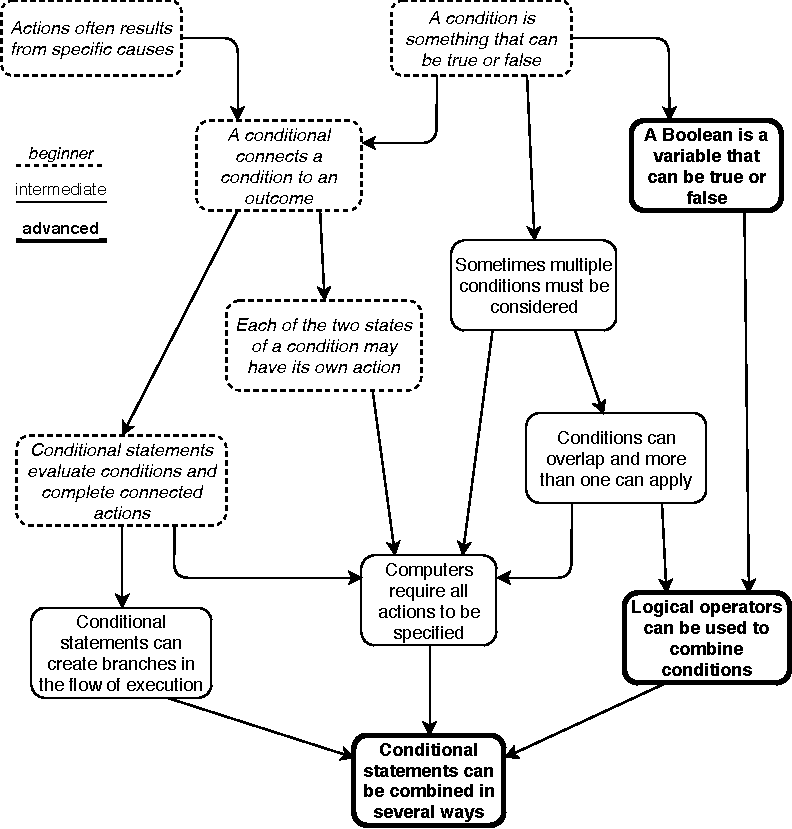
\includegraphics{../docs/fig/conditionals.pdf}
\caption{Learning Trajectory for Conditions (from \cite{Rich2017})}
\label{f:pck-trajectory}
\end{figure}

\section{How Much Are Novices Learning?}\label{s:pck-baseline}

Study after study has shown that teaching evaluations don't correlate
with actual learning outcomes \cite{Star2014,Uttl2017}, so to find out
how much novices are actually learning, we have to use other measures
or do direct studies.  Taking the former approach, roughly two-thirds
of post-secondary students pass their first computing course, with
some variations depending on class size and so on, but with no
significant differences over time or based on language
\cite{Benn2007a,Wats2014}.

Taking the latter approach, \cite{McCr2001} presented a multi-site
international study, which was later replicated by \cite{Utti2013}.
According to the first study, ``{\ldots}the disappointing results
suggest that many students do not know how to program at the
conclusion of their introductory courses.''  More specifically, ``For
a combined sample of 216 students from four universities, the average
score was 22.89 out of 110 points on the general evaluation criteria
developed for this study.''  However, this may say as much about
teachers' expectations as it does about student ability.

A growing number of studies have looked at how prior experience
affects these results.  For example, \cite{Wilc2018} compared the
performance and confidence of novices with and without prior
programming experience in CS1 and CS2.  They found that novices with
prior experience outscored novices without by 10\% in CS1, but those
differences disappeared by the end of CS2.  They also found that women
with prior exposure outperformed their male peers in all areas, but
were consistently less confident in their abilities; we will return to
this issue in \secref{s:motivation-inclusivity}.

\section{Do Languages Matter?}\label{s:pck-language}

The short answer is ``yes'': novices learn to program faster and also
learn more using blocks-based tools like Scratch
(\figref{f:pck-scratch}) that make syntax errors impossible
\cite{Wein2017b}.  And block interfaces encourage exploration in a way
that text does not; like all good tools, Scratch can be learned
accidentally \cite{Malo2010}.

\begin{figure}
\centering
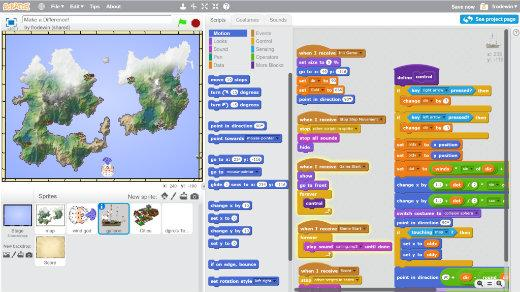
\includegraphics{../docs/fig/scratch.jpg}
\caption{Scratch (from \url{https://opensource.com/article/18/4/designing-game-scratch-open-jam})}
\label{f:pck-scratch}
\end{figure}

\cite{Mlad2017} studied 207 novices learning about loops in Scratch,
Logo, and Python, and found that misconceptions about loops are
minimized when using a block-based language rather than a text-based
language.  What's more, as tasks become more complex (such as using
nested loops) the differences become larger.  Similarly,
\cite{Grov2017} studied 100 middle-school children, they found that
while it was easier for them to assemble programs with blocks than
with text.  However, some concepts are still intrinsically hard, such
as loops that modify variables and logical \texttt{or} (which is often
interpreted as ``one or the other'' rather than ``one or both'').

Scratch has probably been studied more than any other programming
tool, and we know a great deal about how it is used.  For example,
\cite{Aiva2016} analyzed over 250,000 Scratch projects and found among
other things that about 28\% of projects have some blocks that are
never called or triggered.  The authors hypothesize that users may be
using them as a scratchpad to keep bits of code they don't (yet) want
to throw away.

\cite{Wein2017a} went studied people using a tool that allowed them to
switch between blocks and text for programming.  They found that
learners tend to migrate from blocks to text over time, but there are
interesting exceptions.  In two thirds of the cases where learners
shifted from text to blocks, their next action was to add a new type
of command; this may be because browsing available commands is easier
with blocks, or because blocks make syntax errors with unfamiliar new
commands impossible.

Learners also shifted from text to blocks when adding complex control
(e.g., an \texttt{if} with an \texttt{else}), either because syntax
errors are harder, or because the flow of control is immediately
visible.  The authors say, ``While it is often claimed that
blocks-based programming environments offer the advantage of reducing
syntax errors, our findings suggest that blocks also offer information
about what is possible in the space and provide a low-stakes means of
exploring unfamiliar code.''  New tools like
\href{https://www.greenfoot.org/frames/}{Stride} are trying to smooth
the transition between blocks and text even further; when combined
with programming notebooks like \href{http://jupyter.org/}{Jupyter}
and \href{http://stenci.la/}{Stencila}, they may eventually eliminate
the distinction altogether.

\subsection*{Object-Oriented Programming and Functional Programming}

Objects and classes are power tools for experienced programmers, and
many educators advocate an ``objects first'' approach to teaching
programming (though they sometimes disagree on exactly what that means
\cite{Benn2007b}).  \cite{Sorv2014} describes and motivates this
approach, and \cite{Koll2015} describes three generations of tools
designed to support novice programming in object-oriented
environments.

Introducing objects early has a few challenges.  For example,
\cite{Mill2016b} found that most novices using Python had difficulty
with \texttt{self} (which refers to ``this object''): they omitted it
in method definitions, failed to use it when referencing object
attributes, or both.  Object reference errors were also more common
than other errors; the authors speculate that this is partly due to
the difference in syntax between \texttt{obj.method(param)} and
\texttt{def method(self, param)}.  \cite{Rago2017} found something
similar in a study of 86 high school students.  They also found that
high school teachers often weren't clear on the concept either.

Yet another approach is exemplified by the
\href{http://www.bootstrapworld.org/}{Bootstrap project}, which is
based on the \glossref{g:functional-programming}{functional
  programming} paradigm.  This work draws on a rich tradition going
back to languages like Scheme and Lisp, and to classic textbooks like
\cite{Fell2001}, \cite{Frie1995}, and \cite{Abel1996}.  As functional
programming continues to gain ground among professional programmers,
this approach to teaching may continue to grow more popular.

\subsection*{Type Declarations}

Programmers argue a lot about whether variables' data types should
have to be declared or not.  One recent non-educational finding is
\cite{Gao2017}, which selected fixed bugs from public JavaScript
projects, checked out the code from version control just prior to the
fix, manually added type annotations to the buggy code, and then
tested whether strongly-typed variants of JavaScript reported an
error.  They found that about 15\% of bugs are caught, which is either
high or low depending on what answer you wanted in the first place.

However, programming and learning to program are different activities,
and results from the former don't necessarily apply to the latter.
\cite{Endr2014} found that requiring novices to declare variable types
does add some complexity to programs, but it pays off fairly quickly
by acting as documentation for a method's use---in particular, by
forestalling questions about what's available how to use it.

\subsection*{Will Things Get Better?}

\cite{Stef2013} has shown that the creators of programming language
make those languages harder to learn by not doing basic usability
testing.  For example, ``{\ldots}the three most common words for
looping in computer science, \texttt{for}, \texttt{while}, and
\texttt{foreach}, were rated as the three most unintuitive choices by
non-programmers.''  More fundamentally, their work shows that C-style
syntax (as used in Java and Perl) is just as hard for novices to learn
as a randomly-designed syntax, but that the syntax of languages such
as Python and Ruby is significantly easier to learn, and the syntax of
their own language, Quorum, is easier still, because they are testing
each new feature before adding it to the language. (\cite{Stef2017} is
a useful brief summary of what we actually know about designing
programming languages and why we believe it's true.)

However, none of this matters unless designers are willing to take it
into account, and they are often reluctant to do so.  For example,
\cite{Pere2013} compared the actual operation of Git (a popular
version control system) with its users' conceptual model, highlighting
and explaining the many errors and confusion that result from the
differences.  \cite{Pere2016} then used that work to design a more
user-friendly alternative to Git.  The result?

\begin{quote}

  In sharing our research with colleagues{\ldots}we have discovered a
  significant polarization. Experts, who are deeply familiar with the
  product, have learned its many intricacies, developed complex,
  customized workflows, and regularly exploit its most elaborate
  features, are often defensive and resistant to the suggestion that
  the design has flaws. In contrast, less intensive users, who have
  given up on understanding the product, and rely on only a handful of
  memorized commands, are so frustrated by their experience that an
  analysis like ours seems to them belaboring the obvious.

\end{quote}

\section{Can We Give Better Feedback?}\label{s:pck-error}

Incomprehensible error messages are a major source of frustration for
novices (and sometimes for experienced programmers as well).  Several
researchers have explored whether better error messages would help
alleviate this.  For example, \cite{Beck2016} wrote some for the Java
compiler so that instead of:

\begin{verbatim}
C:\stj\Hello.java:2: error: cannot find symbol
        public static void main(string[ ] args){
^
1 error
Process terminated ... there were problems.
\end{verbatim}

\noindent
learners would see:

\begin{verbatim}
Looks like a problem on line number 2.
If "string" refers to a datatype, capitalize the 's'!
\end{verbatim}

\noindent
Novices given these messages made fewer repeated errors and fewer
errors overall.

\cite{Bari2017} went further and used eye tracking to show that
despite the grumblings of compiler writers, people really do read
error messages---in fact, they spend 13--25\% of their time on task
doing this.  Reading error messages turns out to be as difficult as
reading source code, and how difficult it is to read the error
messages strongly predicts task performance.  The inescapable
conclusion is that it really is important to get this right, and that
error messages should be usability tested the same way as any other
interface.

Since interpreting and responding to error message is important,
instructors should give learners exercises that do just that.
\cite{Marc2011} has a rubric for responses to error messages that can
be useful in grading such exercises.

\section{Does Variable Naming Style Matter?}\label{s:pck-code}

\cite{Kern1999} says, ``Programmers are often encouraged to use long
variable names regardless of context. This is a mistake: clarity is
often achieved through brevity.''  Lots of programmers believe this,
and \cite{Hofm2017} found that using full words in variable names led
to an average of 19\% faster comprehension compared to letters and
abbreviations, with no significant difference in speed between single
letters and abbreviations, but didn't look at \emph{which} names were
abbreviated.

For that, we have to turn to \cite{Beni2017}, which found that using
single-letter variable names doesn't affect novice programmers'
ability to modify code.  This may be because novices' programs are
shorter than professionals', but it may also be because some
single-letter variable names have implicit types and meanings: most
programmers assume \texttt{i}, \texttt{j}, and \texttt{n} are
integers, and \texttt{s} is a string, while \texttt{x}, \texttt{y},
and \texttt{z} are either floating-point numbers or integers more or
less equally.

How important is this?  \cite{Bink2012} reported a series of studies
that found that reading and understanding code is fundamentally
different from reading prose: ``{\ldots}the more formal structure and
syntax of source code allows programmers to assimilate and comprehend
parts of the code quite rapidly independent of style.  In
particular{\ldots}beacons and program plans play a large role in
comprehension.''  It also found that experienced developers are
relatively unaffected by identifier style (although again, they didn't
explore \emph{which} variables), and that beginners found CamelCase
easier to read than pothole\_case.  This is surprising because word
spacing improves readability in conventional tasks.  Digging deeper,
``{\ldots}camel casing produces more accurate results.  However, this
correctness comes at a cost as the camel-case style significantly
increases the time needed to correctly detect the correct
identifier.''

\section{Does Visualization Help?}\label{s:pck-visualization}

The idea of visualizing programs is perennially popular, and tools
like \cite{Guo2013} (a web-based tool for visualizing the execution of
Python programs) and \href{http://latentflip.com/loupe/}{Loupe} (which
shows how JavaScript's event loop works) are both popular teaching
aids.  However, we have known for over 20 years that people learn more
from constructing visualizations than they do from viewing
visualizations constructed by others \cite{Stas1998,Ceti2016}, so does
visualization actually helping learning?

To answer this, \cite{Cunn2017} replicated an earlier study of the
kinds of sketching students do when tracing code execution, and
correlations between different kinds and effectiveness.  Different
rates of sketching for different problems indicated that students use
it to externalize cognition; not sketching at all correlates with
lower success, while tracing changes to variables' values by writing
new values near their names as they change was the most effective
strategy.

One possible confounding effect they checked was time: since sketchers
take significantly more time to solve problems, do they do better just
because they think for longer?  The answer is no: there was no
correlation between the time taken and the score achieved.  To the
best of my knowledge, nobody has yet built a debugger that shows
successive values for variables laid out in rows, but this research
suggests that something like that could help.

\begin{callout}{Flowcharts}

  One often-overlooked finding about visualization is that students
  understand flowcharts better than pseudocode \emph{if both are
    equally well structured} \cite{Scan1989}.  Earlier work showing
  that pseudocode outperformed flowcharts used structured pseudocode
  and tangled flowcharts; when the playing field was levelled, novices
  did better with the graphical representation.

\end{callout}

\section{What Else Can We Do to Help?}\label{s:pck-help}

\cite{Viha2014} examined the average improvement in pass rates of
various kinds of intervention in programming classes.  As they
themselves point out, there are many reasons to take their findings
with a grain of salt: the pre-change teaching practices are rarely
stated clearly, the quality of change is not judged, and only 8.3\% of
studies reported negative findings, so either here is positive
reporting bias or the way we're teaching right now is almost the worst
way possible and anything would be an improvement.  It's also worth
remembering that like almost all of the studies discussed in this
chapter, they were only looking at university classes: their findings
may not generalize to other groups.

With all those caveats in mind, they found ten things instructors can
do to improve outcomes.  \figref{f:pck-interventions} shows the
average improvement reported for each type:

\begin{description}

\item[Collaboration:] % (20/34\%)
  Activities that encourage student collaboration either in classrooms
  or labs.

\item[Content Change:] % (36/34\%)
  At least parts of the teaching material was changed or updated.

\item[Contextualization:] % (17/40\%)
  Activities where course content and activities were aligned towards
  a specific context such as games or media.

\item[CS0:] % (7/43\%)
  Creation of a preliminary course to be taken before the introductory
  programming course; could be organized only for some (e.g., at-risk)
  students.

\item[Game Theme:] % (9/18\%)
  A game-themed component was introduced to the course.

\item[Grading Scheme:] % (11/29\%)
  A change in the grading scheme; the most common change was to
  increase the amount of points rewarded from programming activities,
  while reducing the weight of the course exam.

\item[Group Work:] % (7/45\%)
  Activities with increased group work commitment such as team-based
  learning and cooperative learning.

\item[Media Computation:] % (10/48\%)
  Activities explicitly declaring the use of media computation
  (\chapref{s:motivation}).

\item[Peer Support:] % (23/34\%)
  Support by peers in form of pairs, groups, hired peer mentors or
  tutors.

\item[Other Support:] % (9/33\%)
  An umbrella term for all support activities, e.g. increased teacher
  hours, additional support channels, etc.

\end{description}

\begin{figure}
\centering
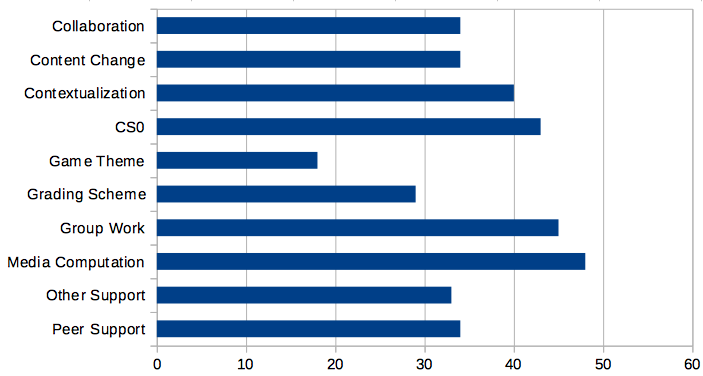
\includegraphics{../docs/fig/interventions.png}
\caption{Effectiveness of Interventions}
\label{f:pck-interventions}
\end{figure}

This list highlights the importance of cooperative learning.
\cite{Beck2013} looked at this specifically over three academic years
in courses taught by two different instructors, and found significant
benefits overall and for many subgroups: they not only had higher
grades, they left fewer questions blank on the final exam, which
indicates greater self-efficacy and willingness to try to debug
things.

As noted earlier, writing code isn't the only way to teach people how
to program.  \cite{Shel2017} reports that having novices work on
computational creativity exercises improves grades at several levels.
A typical exercise is to identify an everyday object (such as nail
clipper, a paper clip, Scotch tape) and describe the object in terms
of its inputs, outputs and functions.  This kind of teaching is
sometimes called ``unplugged'', and the
\href{https://csunplugged.org/en/}{CS Unplugged} site has a collection
of lessons and exercises for doing this.

\section{Exercises}\label{s:pck-exercises}

\exercise{Checking for Common Errors}{individual}{20}

This list of common errors is taken from \cite{Sirk2012}.  Pick three,
and write an exercise for each to check that learners \emph{aren't}
making that mistake.

\begin{description}

  \item[Inverted assignment:] The student assigns the value of the
    left-hand variable to the right-hand side variable, rather than
    the other way around.

  \item[Wrong branch:] Even though the conditional evaluates to
    \texttt{False}, the student jumps to the \texttt{then} clause.

  \item[Wrong \texttt{False}:] As soon as the conditional evaluates to
    \texttt{False} , the student returns \texttt{False} from the
    function.
  
  \item[Executing function instead of defining it:] The student
    believes that a function is executed as it is defined.

  \item[Unevaluated parameters:] The student believes the function
    starts running before the parameters have been evaluated.

  \item[Parameter evaluated in the wrong frame:] The student creates
    parameter variables in the caller's frame, not in the callee's.

  \item[Failing to store return value:] The student does not assign
    the return value in the caller.

  \item[Assignment copies object:] The student creates a new object
    rather than copying a reference.

  \item[Method call without subject:] The student tries to call a
    method from a class without first creating an instance of the
    class.

\end{description}

\exercise{Mangled Code}{pairs}{15}

\cite{Chen2017} describes exercises in which students reconstruct code
that has been mangled by removing comments, deleting or replacing
lines of code, moving lines, inserting extra unneeded lines, and so
on.  Student performance on these correlates strongly with performance
on assessments in which students write code (i.e., whatever
traditional assignments are measuring, these are measuring as well),
but these questions require less (in-person) work to mark.  Take the
solution to a programming exercise you've created in the past, mangle
it in two different ways, and swap with a partner.

\exercise{The Rainfall Problem}{pairs}{10}

Solve the Rainfall Problem in the programming language of your choice
in two different ways. Compare your solutions with those of your
partner.

\exercise{Roles of Variables}{pairs}{15}

Take a short program you have written (5--15 lines) and classify each
of its variables using the categories defined in
\secref{s:pck-programming}.  Compare your classifications with those
of a partner: where did you agree? When you disagreed, did you
understand each other's view?

\exercise{Choose Your Own Adventures}{individual}{10}

Which of the three approaches described in \cite{Sorv2014}
(\secref{s:pck-now}) do you use when teaching? Or is your approach
best described in some other way?

\exercise{What Are You Teaching?}{individual}{10}

Compare the topics you teach to the list developed in \cite{Luxt2017}
(\secref{s:pck-now}).  Which topics do you cover?  What extra topics
do you cover that aren't in their list?

\exercise{Beneficial Activities}{individual}{10}

Look at the list of interventions developed by \cite{Viha2014}
(\secref{s:pck-help}).  Which of these things do you already do in
your classes?  Which ones could you easily add?  Which ones are
irrelevant?

\exercise{Visualizations}{individual}{10}

What visualization do you most like to use when teaching?  Is it a
static image or an animation?  Do you show it to your learners, do
they discover it on their own, or something in between?

\exercise{Misconceptions and Challenges}{small groups}{15}

The \href{http://www.pd4cs.org/}{Professional Development for CS
  Principles Teaching} site includes
\href{http://www.pd4cs.org/mc-index/}{a detailed list of student
  misconceptions and exercises}.  Working in small groups, choose one
section (such as data structures or functions) and go through their
list.  Which of these misconceptions do you remember having when you
were a learner?  Which do you still have?  Which have you seen in your
learners?
